\documentclass[tikz,border=5pt]{standalone}
\usepackage{amsmath, amssymb}
\usetikzlibrary{shapes.geometric, arrows.meta, calc, positioning, decorations.pathmorphing, decorations.pathreplacing}

\begin{document}

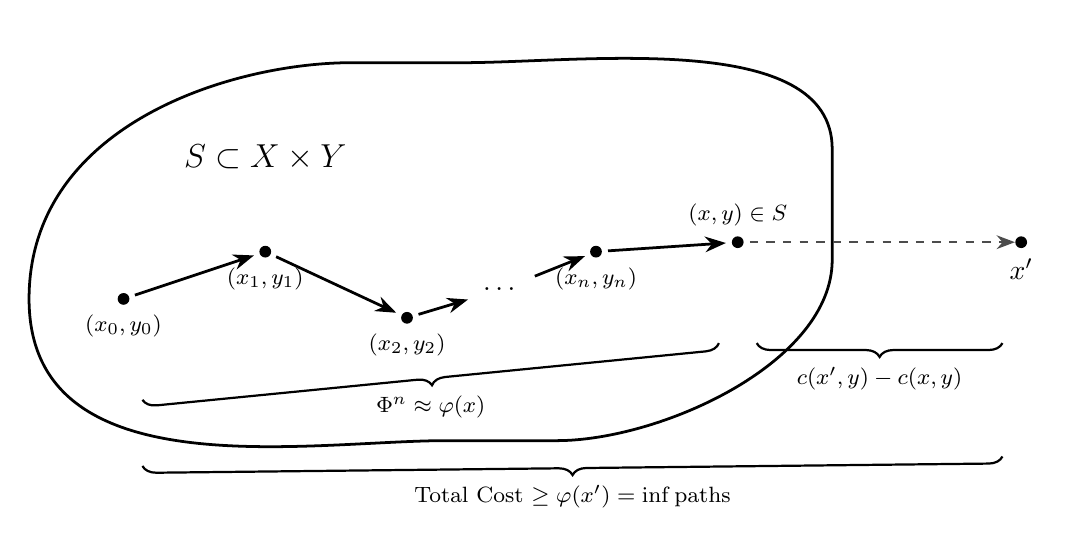
\begin{tikzpicture}[scale=1.2, >=Stealth]

% --- Styles (Black & White / Grayscale) ---
\begin{scope}[xshift=2cm, yshift=0.5cm]
\tikzset{
    setS/.style={fill=white, draw=black, line width=1pt, rounded corners=20pt},
    chainPoint/.style={circle, fill=black, inner sep=1.5pt},
    targetPoint/.style={circle, fill=black, inner sep=1.5pt},
    chainPath/.style={->, black, line width=1pt, shorten >=2pt, shorten <=2pt},
    costEval/.style={->, dashed, black!70, line width=0.8pt, shorten >=2pt, shorten <=2pt},
    % Snake decoration for the 'jump'
    jumpCost/.style={->, thick, black, decorate, decoration={snake, amplitude=.3mm, segment length=2mm, post length=1mm}},
    mathBrace/.style={decorate, decoration={brace, amplitude=5pt, mirror}, thick},
}

% --- The Set S ---
% Shifted UP by 0.5cm to avoid cutoff
\begin{scope}[yshift=0.5cm]
    \filldraw[setS] (-1, 0) to[out=90, in=180] (3, 2.5) to[out=0, in=90] (7.5, 1) to[out=270, in=0] (4, -1.5) to[out=180, in=270] (-1, 0);
    \node[black] at (1.5, 1.5) {\large $S \subset X \times Y$};

    % --- Points in S (The Chain) ---
    % These also move with the scope
    \node[chainPoint, label={below:\footnotesize $(x_0, y_0)$}] (p0) at (0, 0) {};
    \node[chainPoint, label={below:\footnotesize $(x_1, y_1)$}] (p1) at (1.5, 0.5) {};
    \node[chainPoint, label={below:\footnotesize $(x_2, y_2)$}] (p2) at (3, -0.2) {};
    \node (pdots) at (4, 0.1) {$\dots$};
    \node[chainPoint, label={below:\footnotesize $(x_n, y_n)$}] (pn) at (5, 0.5) {};
        % --- The Pivot Point (x,y) in S ---
    \node[chainPoint, label={above:\footnotesize $(x, y) \in S$}] (pxy) at (6.5, 0.6) {};

    
    % Draw Chain Path inside the scope
    \draw[chainPath] (p0) -- (p1);
    \draw[chainPath] (p1) -- (p2);
    \draw[chainPath] (p2) -- (pdots);
    \draw[chainPath] (pdots) -- (pn);
    \draw[chainPath] (pn) -- (pxy);
\node[targetPoint, label={below:$x'$}] (txp) at (9.5, 0.6) {};
\end{scope}

% --- Target Points in X ---
% Kept absolute or adjusted slightly % Moved up slightly to match set shift


% --- Drawing the Paths (Connecting Scope points to Targets) ---


\draw[costEval, ->, shorten >=0pt] (pxy) -- node[below, pos=0.75, font=\footnotesize] {} (txp);

    % --- BRACKETS ---
    % 1. Brace for Phi^n (approximating phi(x)) - spans x0 to xn
    % We use coordinates relative to the nodes.
    \draw[mathBrace] ($(p0.south)+(+0.2,-1)$) -- ($(pxy.south)+(-0.2,-1)$) 
        node[midway, below=5pt, font=\footnotesize] (lbl1) {$\Phi^n \approx \varphi(x)$};
    \draw[mathBrace] ($(pxy.south)+(0.2,-1)$) -- ($(txp.south)+(-0.2,-1)$) 
        node[midway, below=5pt, font=\footnotesize] (lbl1) {$c(x',y) - c(x,y)$};
    % 2. Brace for the extended path (bounding phi(x')) - spans x0 to pivot
    % Placed lower to encompass the first brace
    \draw[mathBrace] ($(p0.south)+(0.2,-1.7)$) -- ($(txp.south)+(-0.2,-2.2)$) 
        node[midway, below=5pt, font=\footnotesize] {Total Cost $\ge \varphi(x') = \inf{\text{paths}}$};
\end{scope}

\end{tikzpicture}
\end{document}